\section{作业}

\subsection{
    {\tt pthread} 函数库可以用来在 {\tt Linux} 上创建线程,请调研了解 {\tt pthread_create} , {\tt pthread_join} , {\tt pthread_exit} 等 API 的使用方法,然后完成以下任务:
}

\subsubsection{
    写一个 {\tt C} 程序,首先创建一个值为$1$到$100$万的整数数组,然后对这$100$万个数求和。请打印最终结果,统计求和操作的耗时并打印。(注:可以使用作业$1$中用到的 {\tt gettimeofday()} 和 {\tt clock_gettime()} 函数测量耗时);
}

我的代码如下所示:

\lstinputlisting[language=C, caption={数组求和}]{code/prog1.c}

下面是统计$10$次并打印的结果:

\begin{figure}[H]
    \centering
    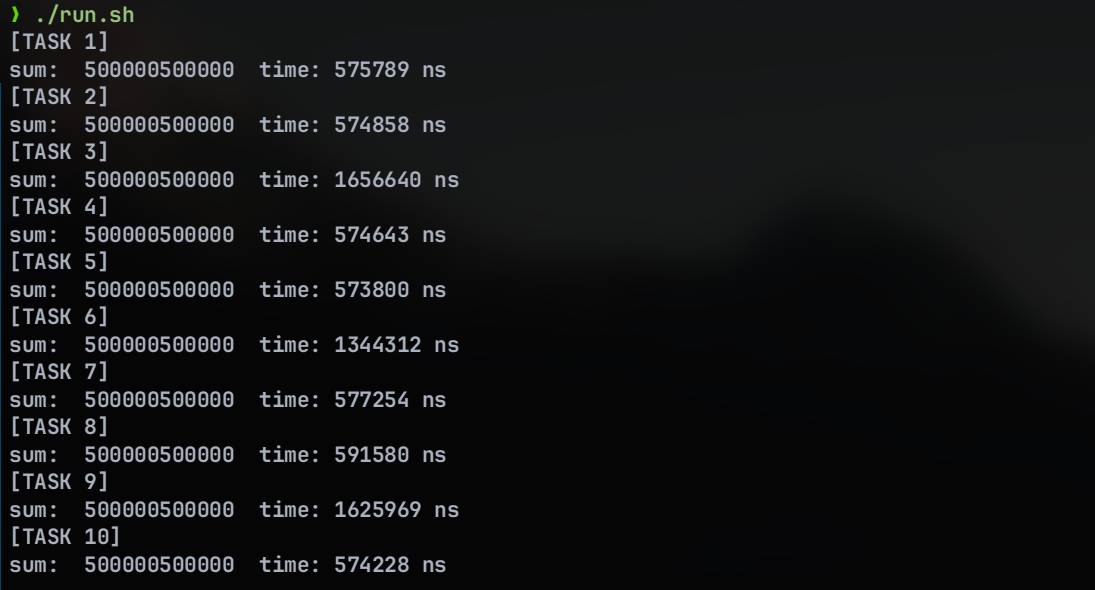
\includegraphics[width=0.8\textwidth]{fig/prog1.png}
    \caption{运行结果}
\end{figure}

平均用时为$866907$纳秒。

\subsubsection{
    在(1)所写程序基础上,在创建完$1$到$100$万的整数数组后,使用 {\tt pthread} 函数库创建 {\tt N} 个线程( {\tt N} 可以自行决定, 且 {\tt N > 1} ),由这 {\tt N} 个线程完成$100$万个数的求和,并打印最终结果。请统计 {\tt N} 个线程完成求和所消耗的总时间并打印。和(1)的耗费时间相比,你能否解释(2)的耗时结果?(注意:可以多运行几次看测量结果)
}

我的代码如下所示,注意用 {\tt long} 类型来存储求和结果,如果使用 {\tt int} 类型会溢出。

\begin{lstlisting}[language=C, caption={多线程求和}]
    ...

    #define ARR_SZ 1000000 /* length of the array */
    #define TIMES  10      /* test times         */
    #define N      4       /* number of threads */

    int arr[ARR_SZ];
    long partial_sums[N];

    typedef struct {
        int start;
        int end;
        int thread_id;
    } thread_data_t;

    static void*
    partial_sum(void* arg) {
        thread_data_t* data = (thread_data_t*)arg;
        long sum = 0;
        for (int i = data->start; i < data->end; i++) {
            sum += arr[i];
        }
        partial_sums[data->thread_id] = sum;
        pthread_exit(NULL);
    }

    static void
    measure_sum(long *sum, long *time)
    {
        ...

        pthread_t threads[N];
        thread_data_t thread_data[N];
        int chunk_size = ARR_SZ / N;

        for (int i = 0; i < N; i++) {
            thread_data[i].start = i * chunk_size;
            thread_data[i].end = (i == N - 1) ? ARR_SZ : (i + 1) * chunk_size;
            thread_data[i].thread_id = i;
            pthread_create(&threads[i], NULL, partial_sum, (void*)&thread_data[i]);
        }

        /* waiting for the threads to end */
        for (int i = 0; i < N; i++) {
            pthread_join(threads[i], NULL);
        }

        long local_sum = 0;
        for (int i = 0; i < N; i++) {
            local_sum += partial_sums[i];
        }
        *sum = local_sum;

        ...
    }

    int
    main(void)
    {
        ...
    }

\end{lstlisting}

在 {\tt N = 4} (示例)的情况下,输出为:

\begin{figure}[H]
    \centering
    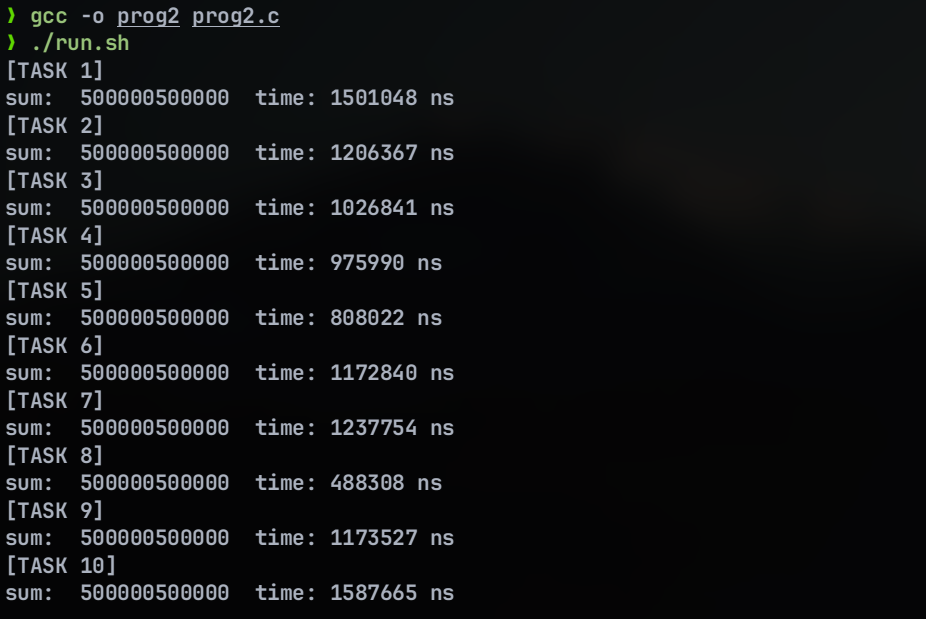
\includegraphics[width=0.8\textwidth]{fig/prog2.png}
    \caption{运行结果}
\end{figure}

对于不同的 {\tt N} ($2$至$16$的偶数),分别统计$10$次并打印,将结果记录在以下表格中:

\begin{table}[H]
    \caption{多线程求和}
    \begin{tabular}{|c|c|c|c|c|c|c|c|c|c|}
    \hline
    test & N=1 & N=2 & N=4 & N=6 & N=8 & N=10 & N=12 & N=14 & N=16 \\ \hline
    1 & 575789 & 1057421 & 1111634 & 457532 & 1323892 & 1136939 & 1515792 & 754861 & 1147827 \\ \hline
    2 & 574858 & 674484 & 1066786 & 1615389 & 1191374 & 1944140 & 1756470 & 1724857 & 3403315 \\ \hline
    3 & 1656640 & 1157499 & 1168025 & 907924 & 1500407 & 1122939 & 863034 & 1417376 & 1450629 \\ \hline
    4 & 574643 & 612377 & 1165201 & 1376822 & 943111 & 2021656 & 1393521 & 1762306 & 831903 \\ \hline
    5 & 573800 & 641166 & 721431 & 855829 & 758768 & 1206046 & 1784008 & 1945444 & 1314023 \\ \hline
    6 & 1344312 & 1295684 & 1067609 & 760620 & 621262 & 2045675 & 1871470 & 1050583 & 1755084 \\ \hline
    7 & 577254 & 615797 & 1150017 & 675828 & 1520860 & 799395 & 437030 & 2154065 & 1438539 \\ \hline
    8 & 591580 & 919412 & 1588089 & 775065 & 1877449 & 706066 & 1280999 & 674625 & 2120364 \\ \hline
    9 & 1625969 & 635315 & 1303151 & 661511 & 1703760 & 883208 & 1247847 & 1921962 & 1848731 \\ \hline
    10 & 574228 & 624170 & 753530 & 808405 & 790683 & 951416 & 1023332 & 1231661 & 1868766 \\ \hline
    average & 866907.3 & 823332.5 & 1109547.3 & 889492.5 & 1223156.6 & 1281748 & 1317350.3 & 1463774 & 1717918.1 \\ \hline
    \end{tabular}
\end{table}

观察表格可以发现,数据的浮动很大。即使是同一个程序,每次运行的时间也会有较大差异,比如 {\tt N=14} 的时候,求和所需时间低至 $674625$ 纳秒,高至 $2154065$ 纳秒。我猜测这是因为线程的创建和销毁会消耗时间,而且线程的调度也是不确定的,我的个人电脑上同时运行的进程较多,情况可能更加复杂。总体看来在 {\tt N=1} 、 {\tt N=2} 、 {\tt N=6} 的时候用时较短,但差别不大。

\subsubsection{
    在(2)所写程序基础上,增加绑核操作,将所创建线程和某个CPU核绑定后运行,并打印最终结果,以及统计{\tt N}个线程完成求和所消耗的总时间并打印。和(1)、(2)的耗费时间相比,你能否解释(3)的耗时结果?(注意:可以多运行几次看测量结果)
}

吸取(2)的经验,为了获得尽可能准确的结果,我选择连续求和 $10000$ 次并取平均值。此外,编译时出现了错误,经过排查后,将 {\tt __USE_GNU} 修改为 {\tt _USE_SOURCE} 得以解决。我的代码如下所示:

\begin{lstlisting}[language=C, caption={多线程求和, 绑核}]
    #define _GNU_SOURCE
    #include <pthread.h>
    #include <sched.h>
    #include <stdio.h>
    #include <stdlib.h>
    #include <time.h>
    #include <unistd.h>
    #include <sys/syscall.h>
    #include <stdint.h>

    #define ARR_SZ 1000000 /* length of the array */
    #define TIMES  10000   /* number of measurements */
    #define N      4       /* number of threads   */

    long arr[ARR_SZ];
    long partial_sums[N];

    typedef struct {
        int start;
        int end;
        int thread_id;
    } thread_data_t;

    static void*
    partial_sum(void* arg) {
        cpu_set_t cpuset; //CPU 核的位图
        CPU_ZERO(&cpuset); //将位图清零
        CPU_SET(N, &cpuset); //设置位图第N 位为 1,表示与 coreN 绑定。N 从 0 开始计数
        sched_setaffinity(pthread_self(), sizeof(cpuset), &cpuset); //将当前线程和 cpuset 位图中指定的核绑定运行
        thread_data_t* data = (thread_data_t*)arg;
        long sum = 0;
        for (int i = data->start; i < data->end; i++) {
            sum += arr[i];
        }
        partial_sums[data->thread_id] = sum;
        pthread_exit(NULL);
    }

    static void
    measure_sum(long *sum, long *time)
    {
        ...
    }

    int
    main(void)
    {
        /* Initialize the array */
        for (long i = 0; i < ARR_SZ; i++) {
            arr[i] = i + 1;
        }
        long total_time = 0;
        long total_sum = 0;
        for (int i = 0; i < TIMES; i++) {
            long time, sum;
            measure_sum(&sum, &time);
            total_time += time;
            total_sum += sum;
        }
        long avg_time = total_time / TIMES;
        long avg_sum = total_sum / TIMES;
        printf("Average sum: %ld, Average time: %ld ns\n", avg_sum, avg_time);
        return 0;
    }

\end{lstlisting}

在 {\tt N = 4} (示例)的情况下,输出为:

\begin{figure}[H]
    \centering
    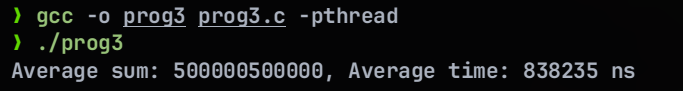
\includegraphics[width=0.8\textwidth]{fig/prog3.png}
    \caption{运行结果}
\end{figure}

因为(2)中发现测量结果有较大浮动,对于不同的 {\tt N} ($1$,以及$2$至$16$的偶数),我用最新的代码重新测试了包含前两问,结果如下:

\begin{table}[H]
    \caption{多线程求和用时}
    \begin{tabular}{|c|c|c|c|c|c|c|c|c|c|}
    \hline
    线程数 & N=1 & N=2 & N=4 & N=6 & N=8 & N=10 & N=12 & N=14 & N=16 \\ \hline
    无绑核 & 760187 & 406816 & 297994 & 332141 & 374823 & 424786 & 551917 & 739925 & 903712 \\ \hline
    绑核 & 1391204 & 1143213 & 829370 & 603649 & 526281 & 533703 & 607141 & 725278 & 873525 \\ \hline
    \end{tabular}
\end{table}

为了便于分析理解,我将上述数据绘制成图表:

\begin{figure}[H]
    \centering
    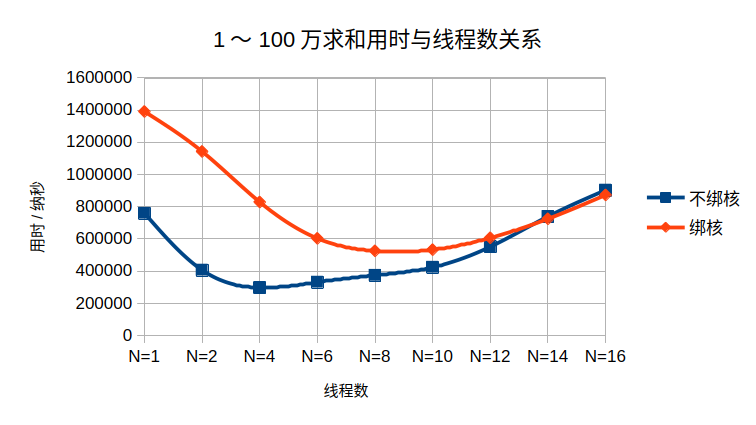
\includegraphics[width=1\textwidth]{fig/chart.png}
    \caption{多线程求和用时}
\end{figure}

显而易见,只要测量的次数足够多,就能尽可能避免测试时因为CPU环境复杂造成的误差,更有助于统计分析。从图表中可以总结出以下规律:

\begin{enumerate}
    \item 无论是否绑核,随着线程数的增加,求和所需时间变化趋势相同,都是先减少再增加的。很有可能是因为在线程数较少的时候,求和所占用时间的影响超过了线程创建、销毁以及调度的影响,因此随着线程数增加,可以显著地提高效率,充分利用多核CPU的并行计算能力;但是线程数过多的时候,线程的创建和销毁所消耗时间超过了求和本身所占时间,线程的调度也更加复杂,反而会浪费更多时间。
    \item 总体来看,绑核时求和所需时间反而更长。可能是因为绑核将线程固定在特定核心上,从而导致调度灵活性降低;而不绑核更容易找到资源闲置的核心,从而提高了计算效率。此外,不绑核时大约在 $N=4$ 时求和所需时间最短,绑核时大约在 $N=8$ 时求和所需时间最短,也很有可能是因为绑核在线程数少时调度灵活性降低,不利于发挥优势。
\end{enumerate}


\subsection{
    请调研了解{\tt pthread_create},{\tt pthread_join},{\tt pthread_exit}等 API 的使用方法后,完成以下任务:
}

\subsubsection{
    写一个{\tt C}程序,首先创建一个有$100$万个元素的整数型空数组,然后使用{\tt pthread}创建{\tt N}个线程({\tt N}可以自行决定, 且{\tt N > 1}),由这{\tt N}个线程完成前述$100$万个元素数组的赋值(注意:赋值时第{\tt i}个元素的值为{\tt i}。最后由主进程对该数组的$100$万个元素求和,并打印结果,验证线程已写入数据。
}

第二题与第一题的(2)十分类似,主要区别在于一个统计的是多线程求和的时间,另一个统计的是多线程赋值的时间。我的代码如下所示(关键注释已经添加至代码中):

\lstinputlisting[language=C, caption={多线程赋值}]{code/prog4.c}

执行结果如下:

\begin{figure}[H]
    \centering
    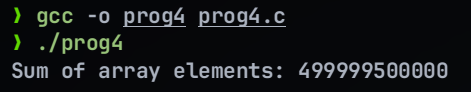
\includegraphics[width=0.6\textwidth]{fig/prog4.png}
    \caption{运行结果}
\end{figure}
